\let\negmedspace\undefined
\let\negthickspace\undefined
\documentclass[journal]{IEEEtran}
\usepackage[a5paper, margin=10mm, onecolumn]{geometry}
%\usepackage{lmodern} % Ensure lmodern is loaded for pdflatex
\usepackage{tfrupee} % Include tfrupee package

\setlength{\headheight}{1cm} % Set the height of the header box
\setlength{\headsep}{0mm}     % Set the distance between the header box and the top of the text

\usepackage{gvv-book}
\usepackage{gvv}
\usepackage{cite}
\usepackage{amsmath,amssymb,amsfonts,amsthm}
\usepackage{algorithmic}
\usepackage{graphicx}
\usepackage{textcomp}
\usepackage{xcolor}
\usepackage{txfonts}
\usepackage{listings}
\usepackage{enumitem}
\usepackage{mathtools}
\usepackage{gensymb}
\usepackage{comment}
\usepackage[breaklinks=true]{hyperref}
\usepackage{tkz-euclide} 
\usepackage{listings}
% \usepackage{gvv}                                        
\def\inputGnumericTable{}                                 
\usepackage[latin1]{inputenc}                                
\usepackage{color}                                            
\usepackage{array}                                            
\usepackage{longtable}                                       
\usepackage{calc}                                             
\usepackage{multirow}                                         
\usepackage{hhline}                                           
\usepackage{ifthen}                                           
\usepackage{lscape}

\begin{document}

\bibliographystyle{IEEEtran}
\vspace{3cm}

\title{9-9.3-14}
\author{EE24BTECH11063 - Y.Harsha Vardhan Reddy}
% \maketitle
% \newpage
% \bigskip
{\let\newpage\relax\maketitle}

\renewcommand{\thefigure}{\theenumi}
\renewcommand{\thetable}{\theenumi}
\setlength{\intextsep}{10pt} % Space between text and floats


\numberwithin{equation}{enumi}
\numberwithin{figure}{enumi}
\renewcommand{\thetable}{\theenumi}
\textbf{Question}:\\
Find the area of the smaller region bounded by the ellipse $\frac{x^2}{9}$+$\frac{y^2}{4}$=1 and the line $\frac{x}{3}$+$\frac{y}{2}$=1.
\\
\solution
\begin{table}[h!]    
  \centering
  \begin{tabular}[12pt]{ |c| c|}
    \hline
    \textbf{Variable} & \textbf{Description}\\ 
    \hline
    $V_1,u_1,f_1$ & Parameters of Parabola \\
    \hline 
    $V_2,u_2,f_2$ & Parameters of circle \\
    \hline
     $P_1,P_2$ & Points of intersection \\
     \hline
     $A$ & Area between the conics \\
    \hline
\end{tabular}

  \caption{Variables Used}
  \label{tab1-1.2-20}
\end{table}
The parameters of given conic,
\begin{align}
	V=\myvec{\frac{1}{9} & 0 \\ 0 & \frac{1}{4}} \\
	u=\myvec{0 \\ 0} \\
	f=0
\end{align}
for the line ,
\begin{align}
h=\myvec{0\\2}\\
m=\myvec{3\\-2}
\end{align}
By Solving we get points of intersection as 
\begin{align}
	\myvec{3\\0},\myvec{0\\ 2}
\end{align}
Area can be evaluated as
\begin{align}
	\int_{0}^{3} \brak{f\brak{x}-g\brak{x}} \, dx \\
	\int_{0}^{3} \brak{2\sqrt{1-\frac{x^2}{9}}-\brak{-\frac{2}{3}x+2}} \, dx
\end{align}
By simplifying area enclosed comes to be 1.71 sq.units
\begin{figure}[h!]
   \centering
   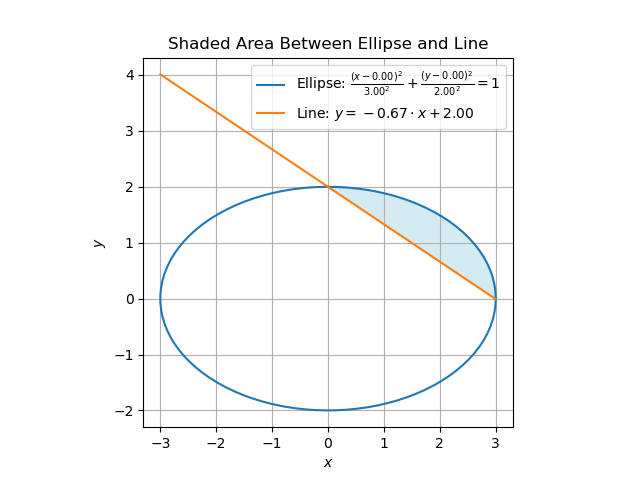
\includegraphics[width=\linewidth]{figs/figure_1.png}
   \label{stemplot}
   \caption{}
\end{figure}





\end{document}
